\documentclass[12pt, twoside]{article}
\usepackage[letterpaper, margin=1in, headsep=0.5in]{geometry}
\usepackage[english]{babel}
\usepackage[utf8]{inputenc}
\usepackage{amsmath}
\usepackage{amsfonts}
\usepackage{amssymb}
\usepackage{tikz}
%\usetikzlibrary{quotes, angles}

\usepackage{graphicx}
\usepackage{enumitem}
\usepackage{multicol}

\usepackage{fancyhdr}
\pagestyle{fancy}
\fancyhf{}
\renewcommand{\headrulewidth}{0pt} % disable the underline of the header

\fancyhead[RE]{\thepage}
\fancyhead[RO]{\thepage \\ Name: \hspace{3cm}}
\fancyhead[LO]{BECA / Dr. Huson / 10th Grade Geometry\\* Unit 5: Transformation, dilation, and scale \\* 13 November 2019}

\begin{document}
\subsubsection*{5.6 Do Now: Regents dilation problems}
 \begin{enumerate}


\item After a dilation centered at the origin, the image of $\overline{CD}$ is $\overline{C'D'}$. If the coordinates of the endpoints of these segments are $C(6,-4)$, $D(2,-8)$, $C'(9,-6)$, and $D'(3,-12)$, find the scale factor of the dilation.\\[0.25cm]
Make a table of coordinate pairs and graph the two line segments,  $\overline{CD}$ and  $\overline{C'D'}$, on the set of axes below.
  \begin{flushright}
    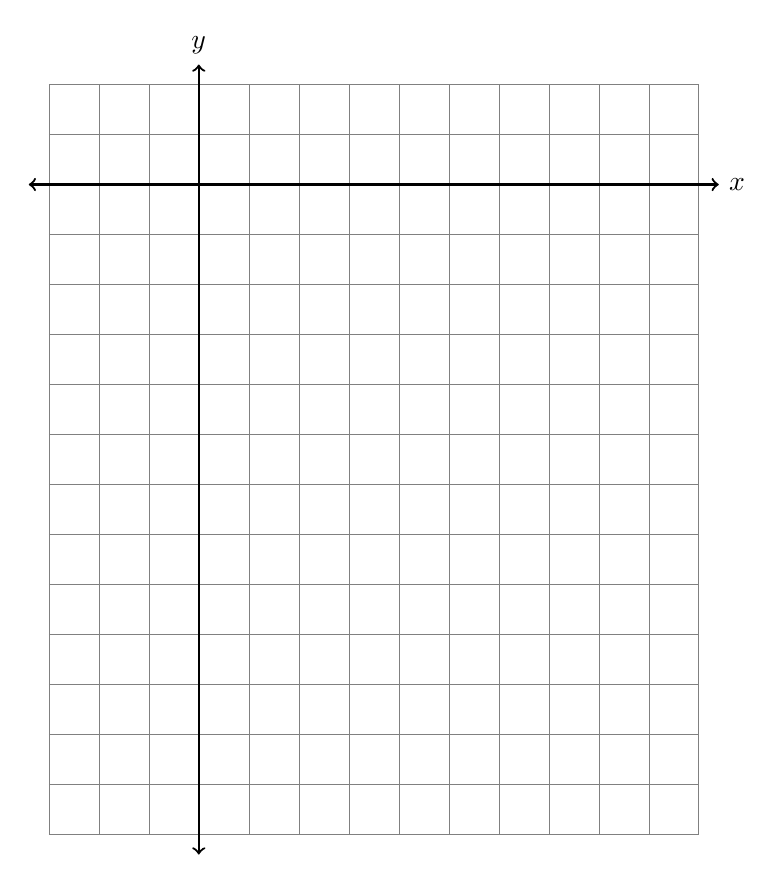
\begin{tikzpicture}[scale=.635]
      \draw [help lines] (-3,-13) grid (10,2);
      \draw [thick, <->] (-3.4,0) -- (10.4,0) node [right] {$x$};
      \draw [thick, <->] (0,-13.4)--(0,2.4) node [above] {$y$};
    \end{tikzpicture}
  \end{flushright}


 \item In the diagram below of $\triangle ABC$, $D$ is a point on $\overline{BA}$, $E$ is a point on $\overline{BC}$, and $\overline{DE}$ is drawn. \\*[2pt] 
 If $BD=5$, $DA=12$, and $BE=7$, what is the length of $\overline{BC}$ so that $\overline{AC} \parallel \overline{DE}$?
 
 \begin{flushright}
     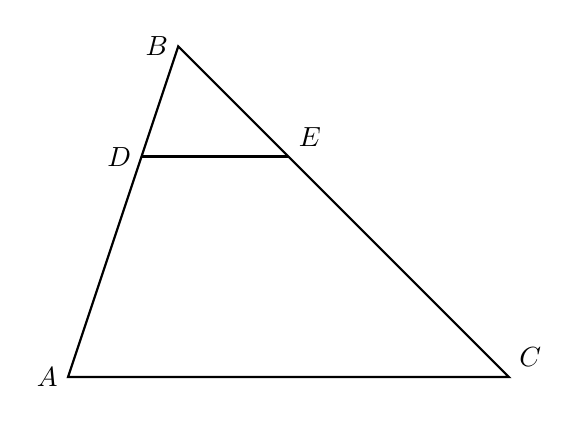
\begin{tikzpicture}[scale=0.7]
       \draw [thick]
       (0,0)node[left]{$A$}--
       (8,0)node[above right]{$C$}--
       (2,6)node[left]{$B$}--cycle;
       \draw [thick]
       (4/3,4)node[left]{$D$}--
       (4,4)node[above right]{$E$};
     \end{tikzpicture}
   \end{flushright}


\newpage


\end{enumerate}
\end{document}
